\documentclass{beamer}
\usetheme[pageofpages=of,% String used between the current page and the
                         % total page count.
          bullet=circle,% Use circles instead of squares for bullets.
          titleline=true,% Show a line below the frame title.
          alternativetitlepage=true,% Use the fancy title page.
       %   titlepagelogo=logo-polito,% Logo for the first page.
       %   watermark=watermark-polito,% Watermark used in every page.
       %   watermarkheight=100px,% Height of the watermark.
       %   watermarkheightmult=4,% The watermark image is 4 times bigger
                                % than watermarkheight.
          ]{Torino}

\setbeamertemplate{footline}{
  \begin{beamercolorbox}[wd=\paperwidth,ht=1ex,dp=1ex]{footline}
    \vspace{5pt} \hspace{1em} \insertframenumber/\inserttotalframenumber
  \end{beamercolorbox}
}

\author{Brendon J. Brewer}
\title{STATS 331 -- Introduction to Bayesian Statistics}
\institute{The University of Auckland}
\date{}


\linespread{1.3}
\usepackage{minted}
\usepackage[utf8]{inputenc}
\usepackage{dsfont}
\newcommand{\given}{\,|\,}
\newcommand{\balpha}{\boldsymbol{\alpha}}
\newcommand{\bmu}{\boldsymbol{\mu}}


\begin{document}

\frame{\titlepage}

\begin{frame}
\begin{center}

\includegraphics[width=0.7\textwidth]{images/dad.png}
\end{center}

\end{frame}


\begin{frame}
\centering
\Large
Two unrelated subjects:
One-way ANOVA and Posterior Predictive Checks

\end{frame}


\begin{frame}
\frametitle{Reminder of T-Tests}

\begin{center}
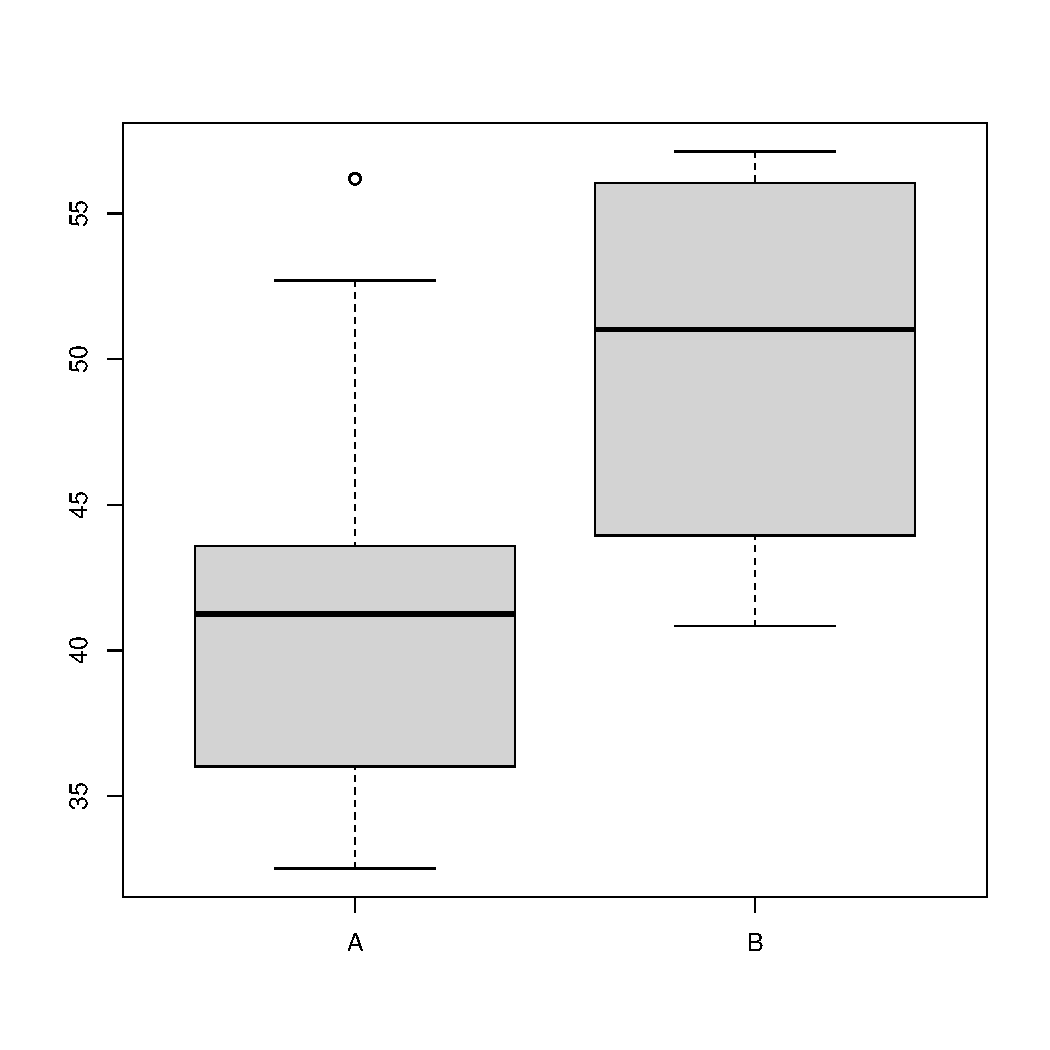
\includegraphics[width=0.6\textwidth]{images/widgets_boxplot.pdf}
\end{center}

\end{frame}

\begin{frame}[fragile]
\frametitle{Reminder of T-Test Model 3}
Recall T-Test Model 3, which modelled the idea that the group mean
parameters $\mu_1$ and $\mu_2$ might be close together or far apart, but not
exactly equal. The priors were hierarchical:\pause
\footnotesize

\begin{minted}{r}
grand_mean ~ dnorm(0, 1/1000^2)
log_diversity ~ dunif(-10, 10)
diversity <- exp(log_diversity)
mu1 ~ dnorm(grand_mean, 1/diversity^2)
mu2 ~ dnorm(grand_mean, 1/diversity^2)
log_sigma ~ dunif(-10, 10)
sigma <- exp(log_sigma)
\end{minted}

\end{frame}


\begin{frame}[fragile]
\frametitle{Reminder of T-Test Model 3}
(Zoomed in)
\begin{center}
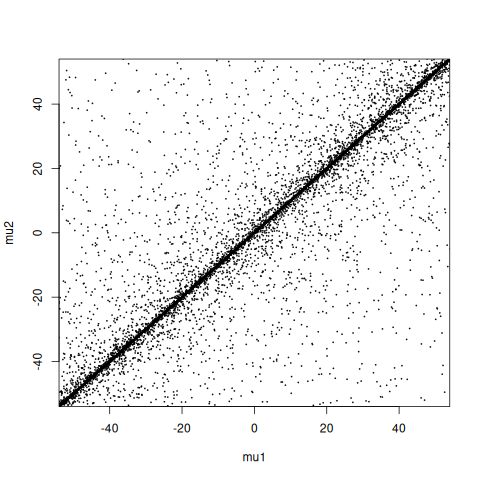
\includegraphics[width=0.5\textwidth]{images/ttest_prior3.png}
\end{center}

\end{frame}



\begin{frame}[fragile]
\frametitle{Reminder of T-Test Model 3}
The sampling distribution/likelihood part of T-Test Model 3 was very
formulaic:

\begin{minted}{r}
for(i in 1:N1)
{
    x1[i] ~ dnorm(mu1, 1/sigma^2)
}
for(i in 1:N2)
{
    x2[i] ~ dnorm(mu2, 1/sigma^2)
}
\end{minted}

\end{frame}



\begin{frame}[fragile]
\frametitle{Example Data: More Groups}

\begin{columns} % Create two columns
    \column{0.4\textwidth} % Left column (50% width)
    \begin{itemize}
    \item Masses of starlings, in grams, at four different locations.
    \item The locations don't have an order to them, so we are not doing
          simple linear regression.
    \end{itemize}

    \column{0.6\textwidth} % Right column (50% width)
    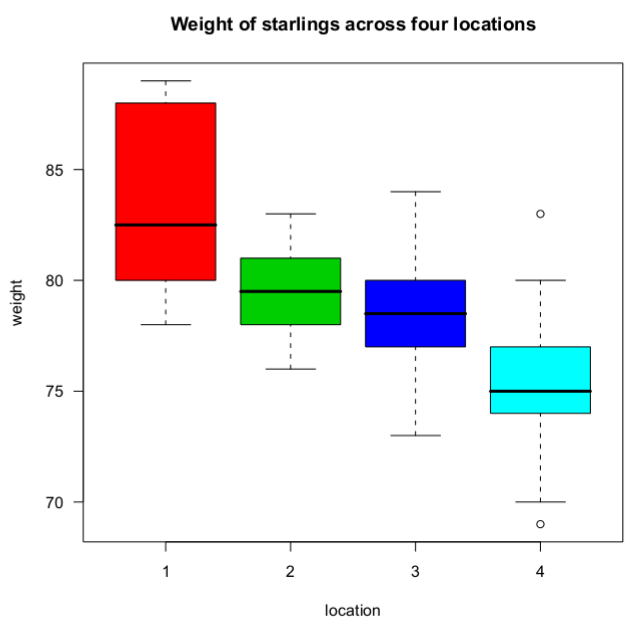
\includegraphics[width=1\linewidth]{images/starling.png}
 \end{columns}


\end{frame}


\begin{frame}[fragile]
\frametitle{Starling Data: CSV File}
The data is in a different format compared to before (all masses are in one
vector).
\begin{minted}{r}
> data = read.csv("starling.csv")
> head(data)
  location  Y
1        1 78
2        1 88
3        1 87
4        1 88
5        1 83
6        1 82
\end{minted}

\end{frame}

\end{document}

